\chapter{Comparação entre os modelos}

\begin{figure}[h]
    \caption{Probabilidade do jogador usar \textit{silêncio} no dilema do prisioneiro em diferentes grafos estrela com matriz de pagamentos FAZER REF e, para jogadores hiper-racionais, matriz de preferências FAZER REF. Na primeira coluna temos a distribuição de estratégias para $t=0$ e nas demais temos a distribuição para $t=100$ nos grafos dados.}
    \centerline{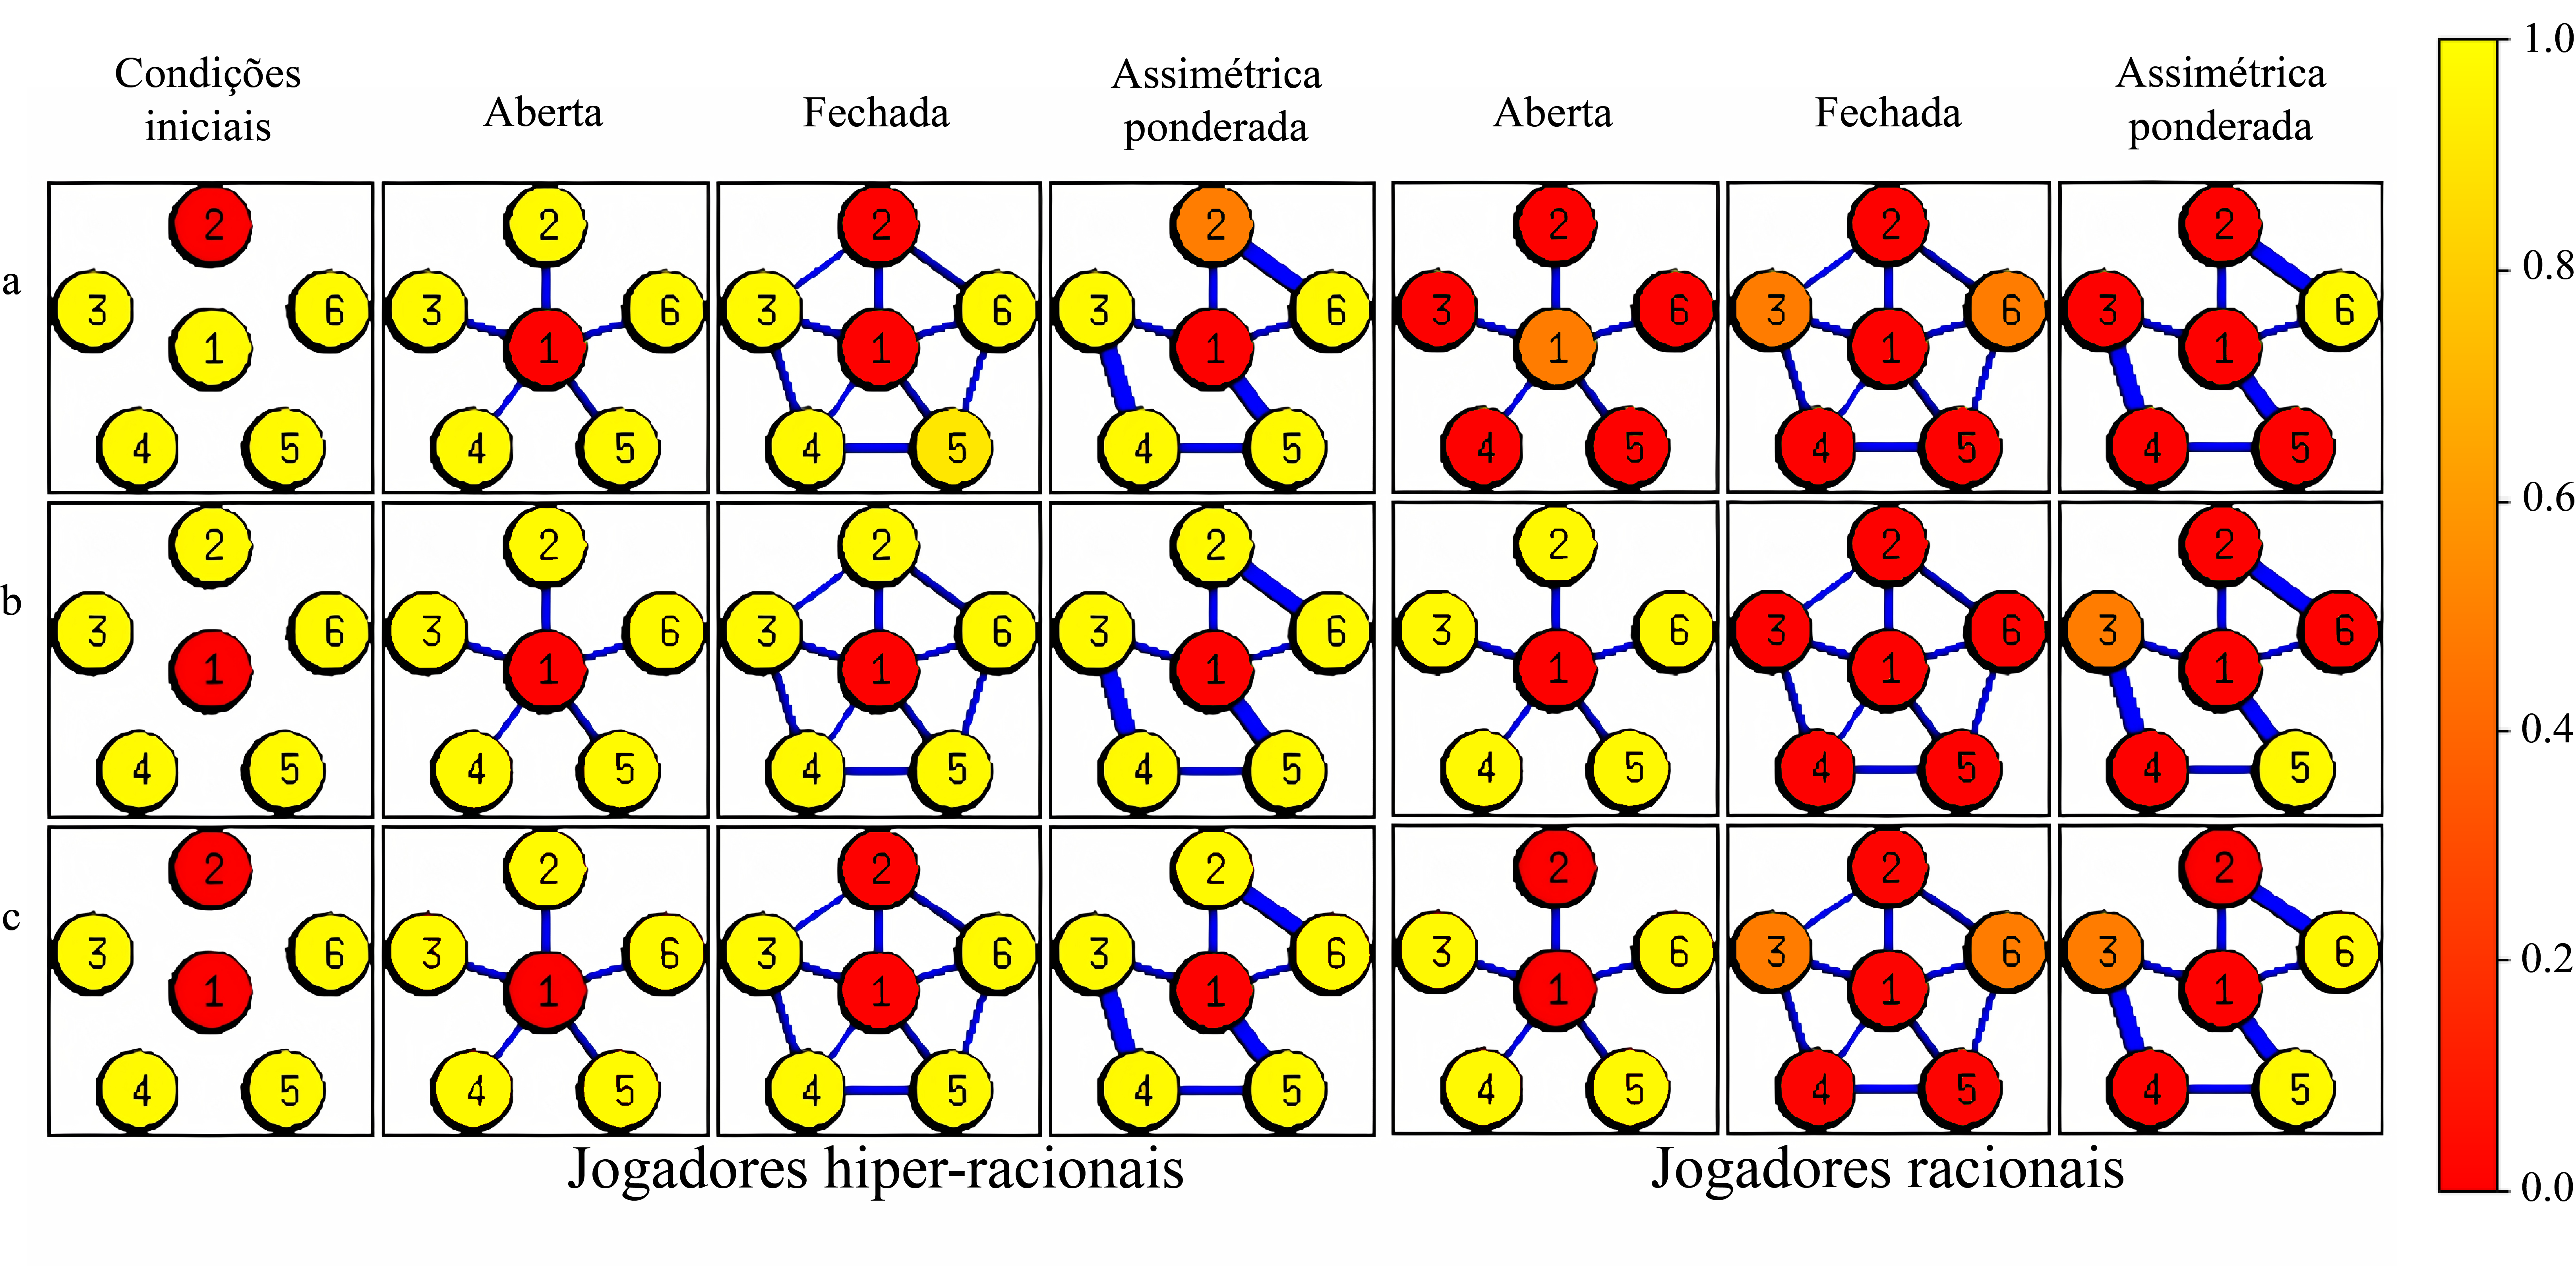
\includegraphics[scale=0.27]{./img/prisoner-control.png}}
    \label{fig:prisoner-control.png}
\end{figure}

\begin{figure}[h]
    \caption{Probabilidade do jogador usar \textit{silêncio} no dilema do prisioneiro em diferentes grafos estrela com matriz de pagamentos FAZER REF e, para jogadores hiper-racionais, matriz de preferências FAZER REF. Na primeira coluna temos a distribuição de estratégias para $t=0$ e nas demais temos a distribuição para $t=50$ nos grafos dados.}
    \centerline{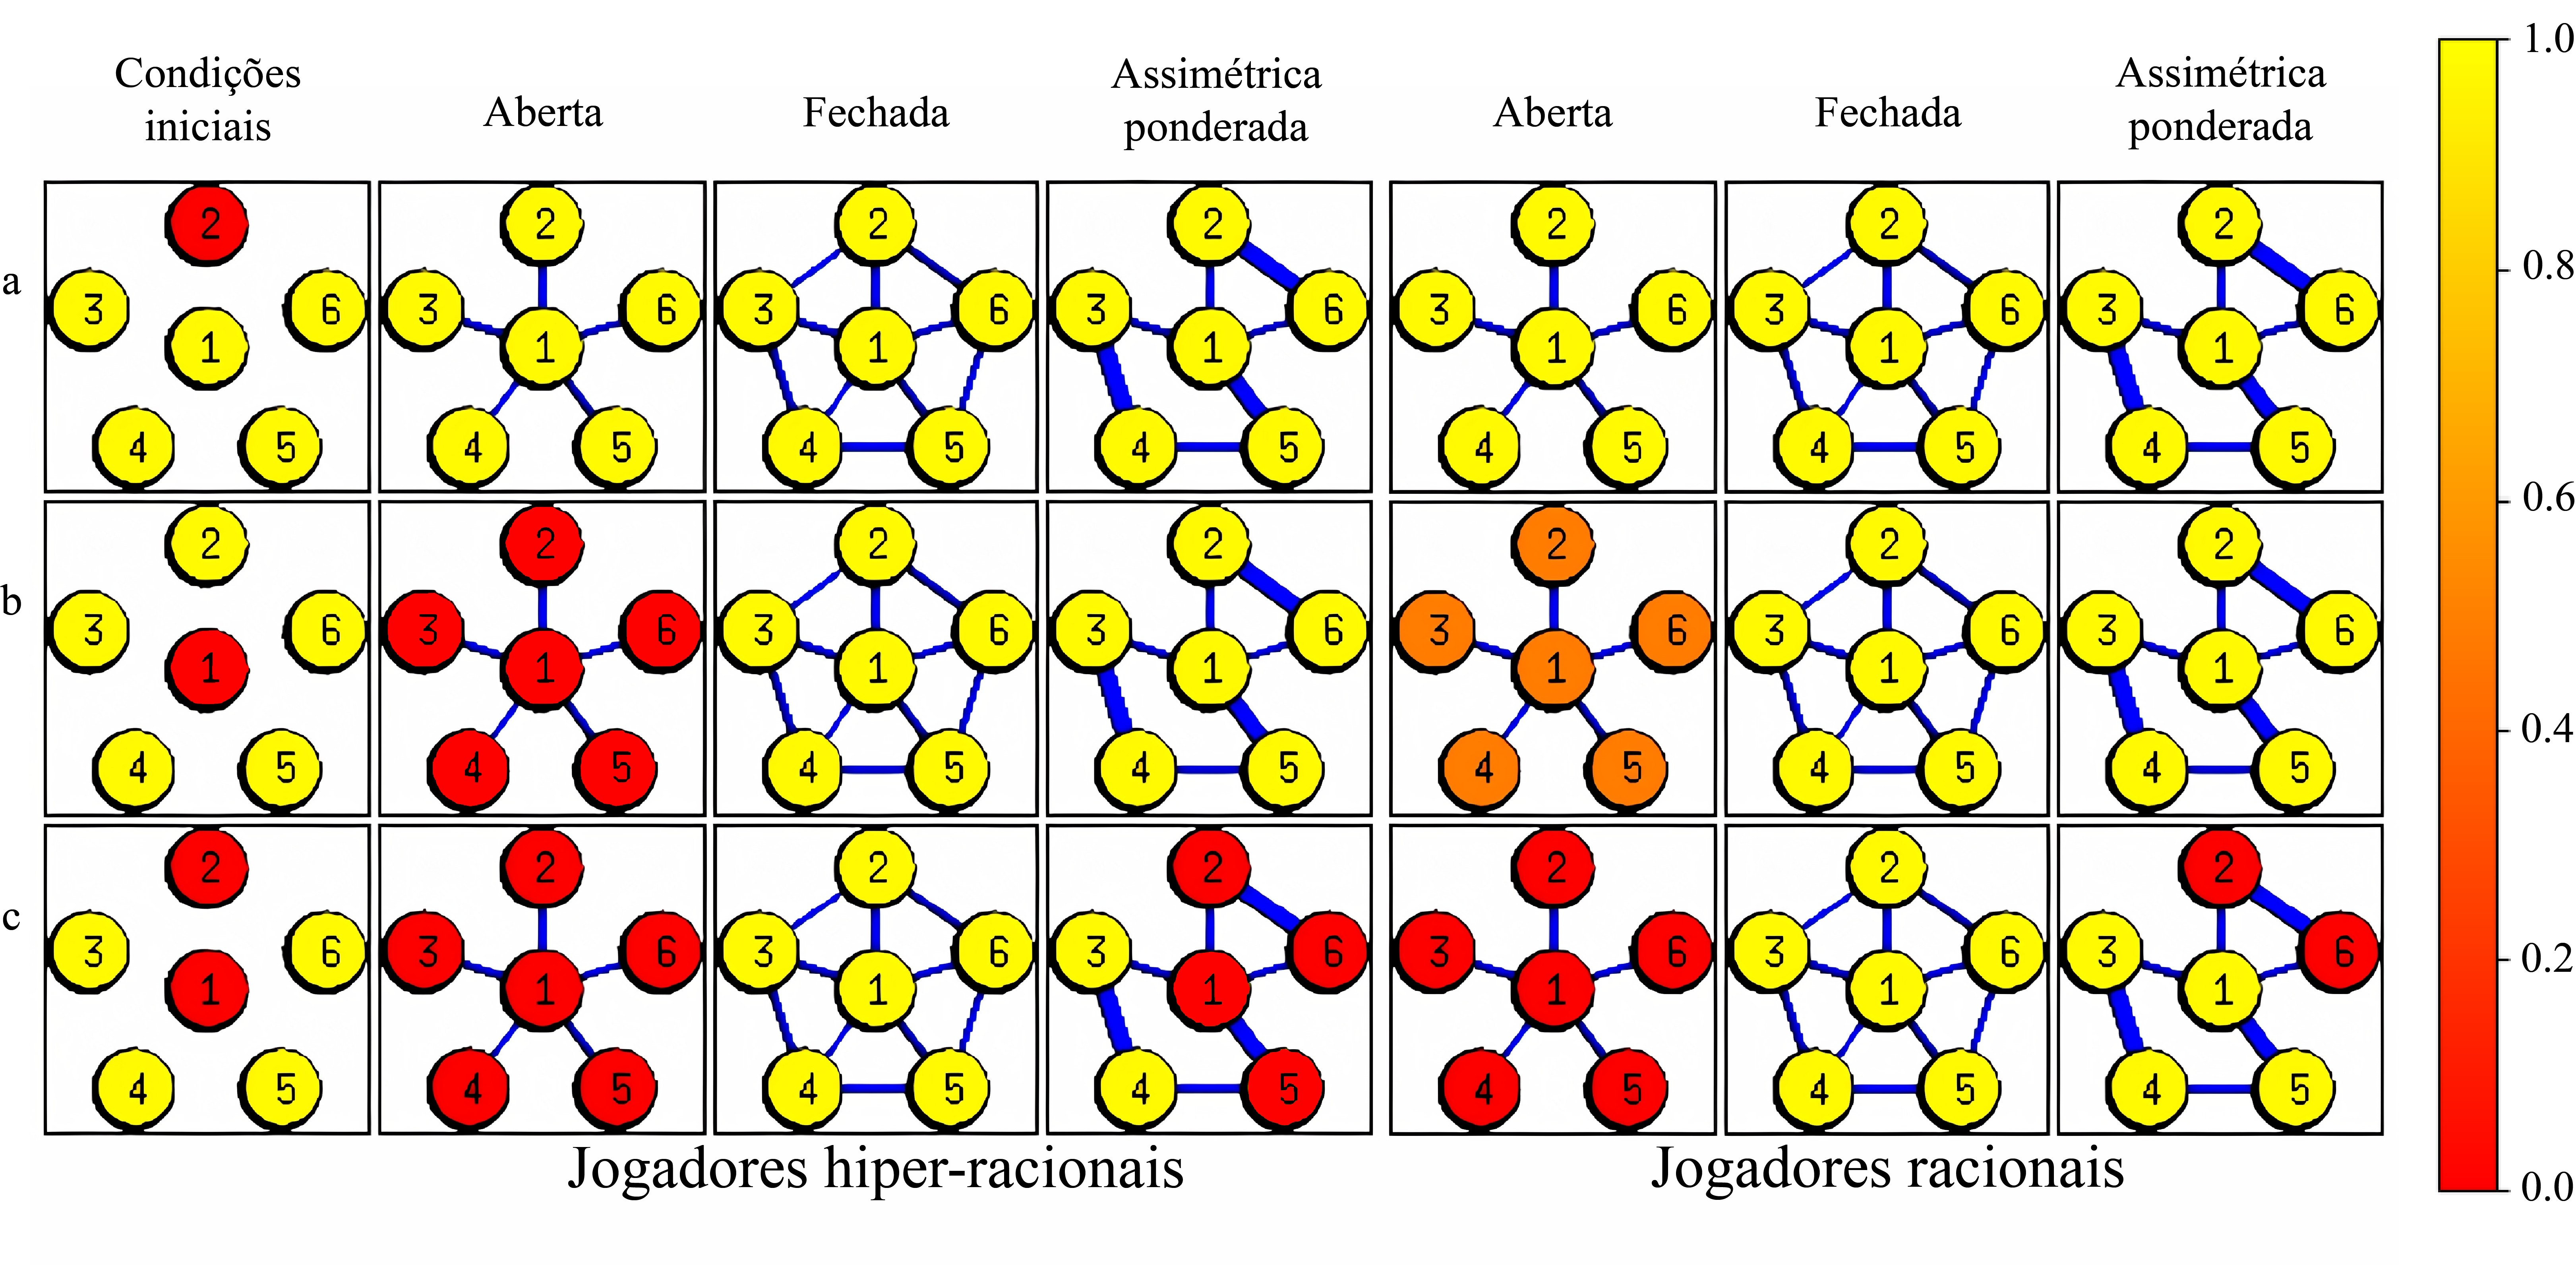
\includegraphics[scale=0.27]{./img/bistability-control.png}}
    \label{fig:bistability-control.png}
\end{figure}

\begin{figure}[h]
    \caption{Probabilidade do jogador usar \textit{silêncio} no dilema do prisioneiro em diferentes grafos estrela com matriz de pagamentos FAZER REF e, para jogadores hiper-racionais, matriz de preferências FAZER REF. Na primeira coluna temos a distribuição de estratégias para $t=0$ e nas demais temos a distribuição para $t=50$ nos grafos dados.}
    \centerline{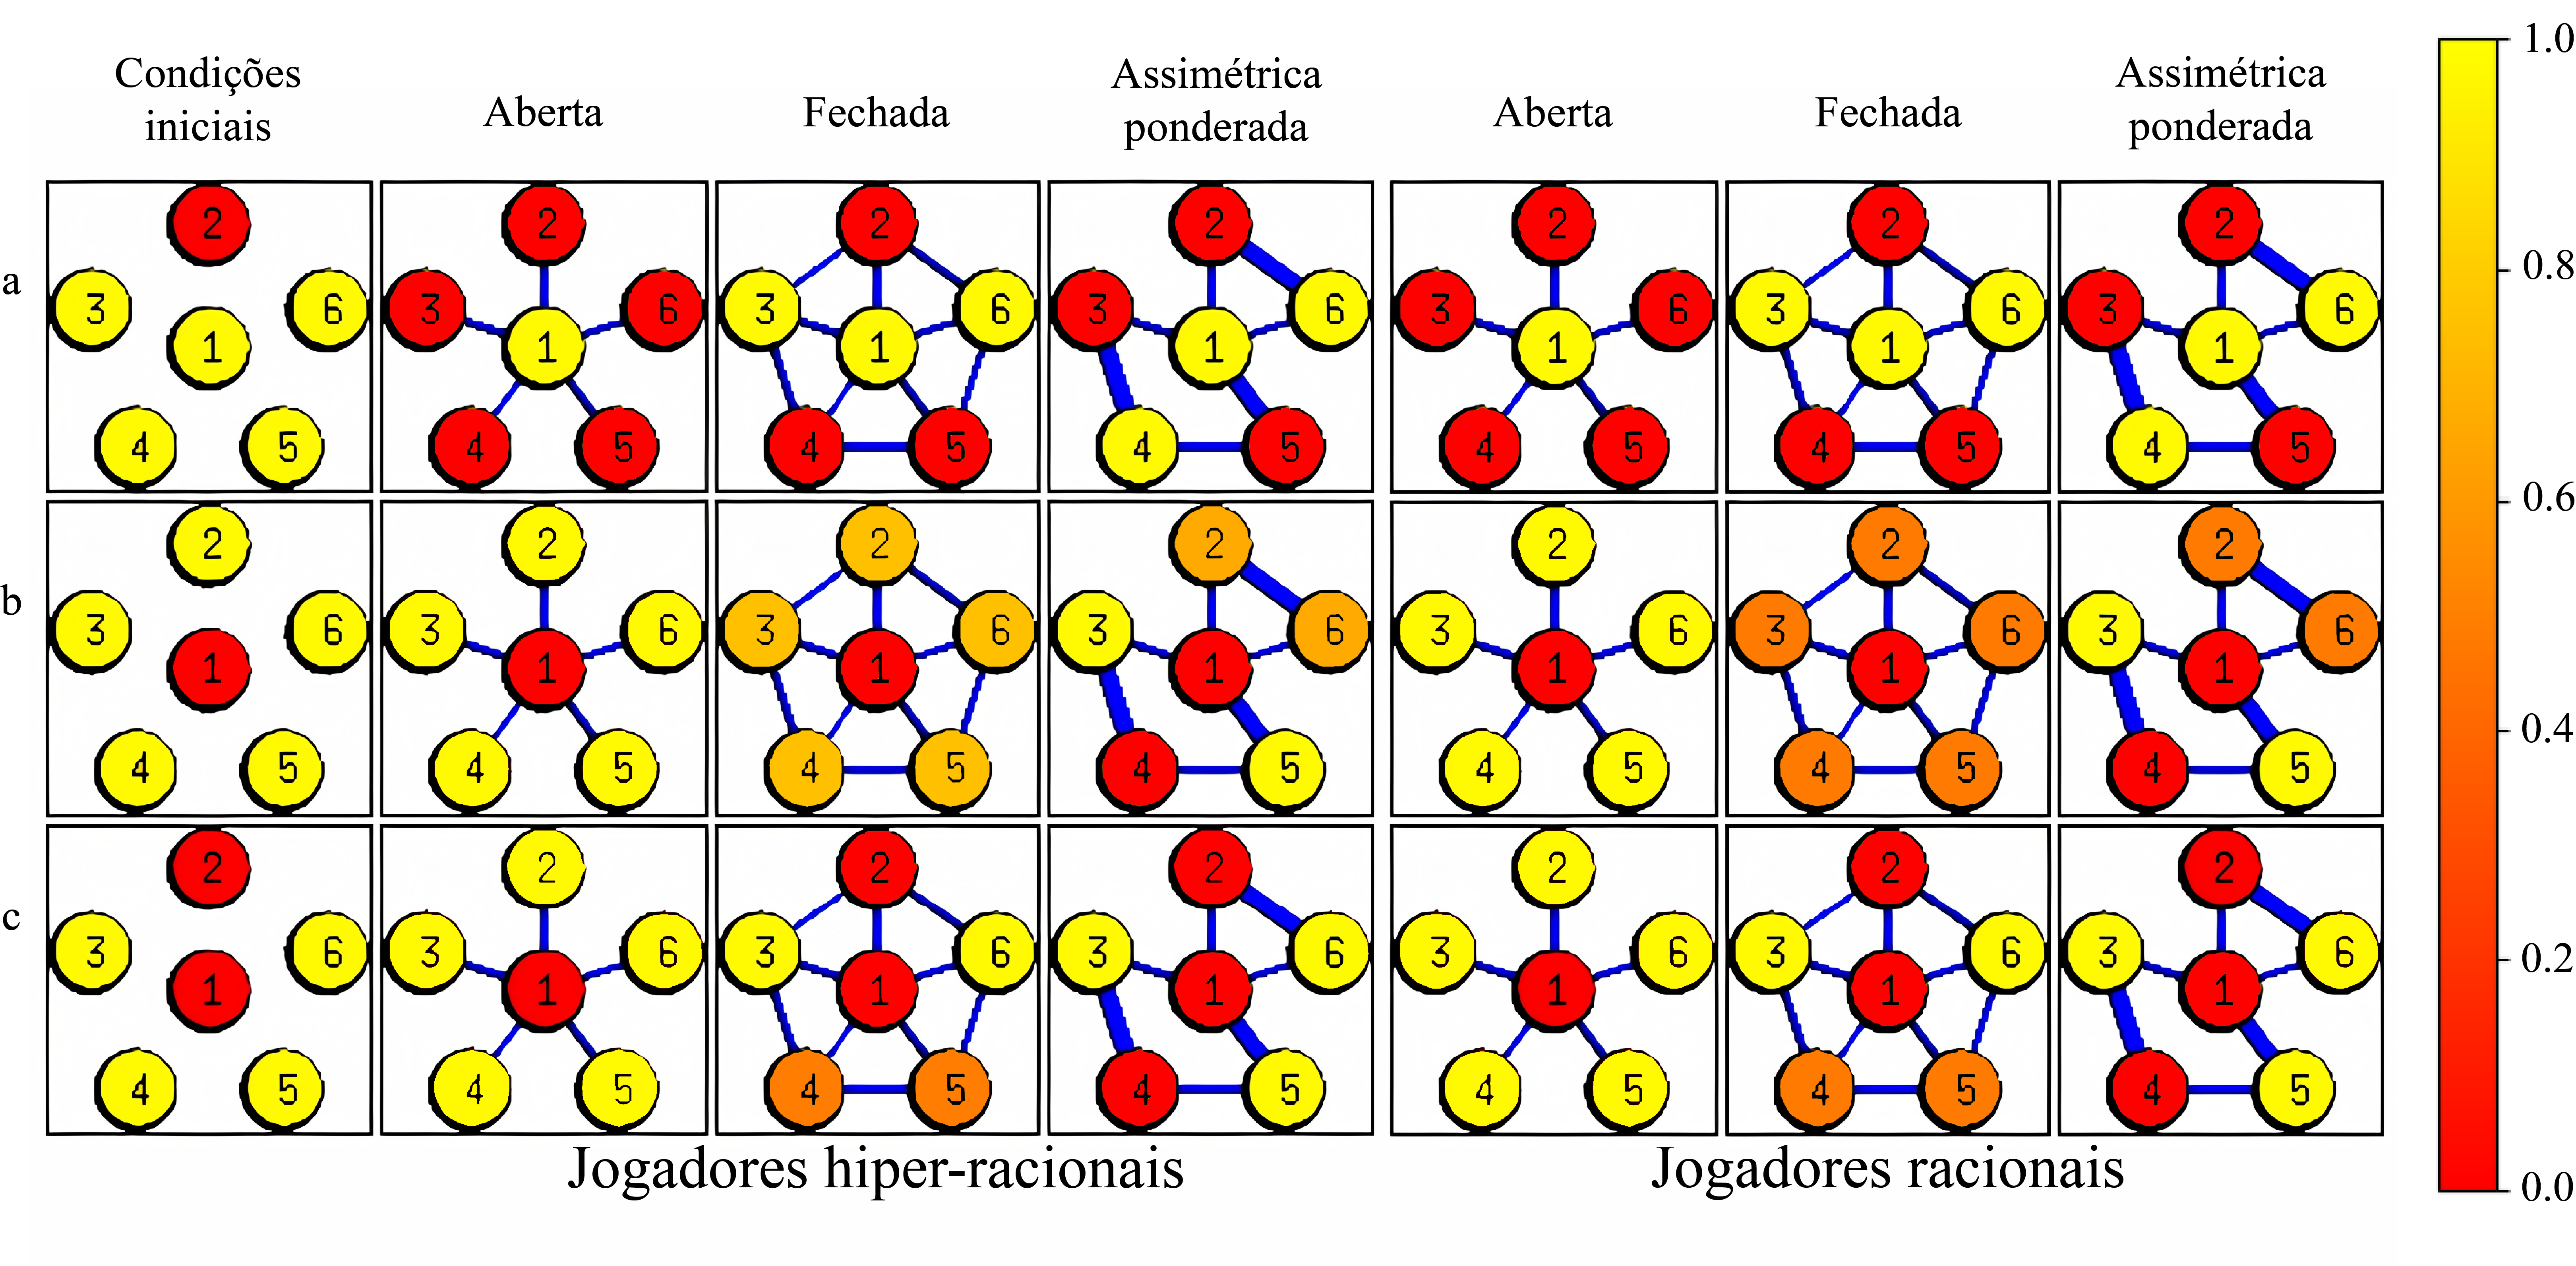
\includegraphics[scale=0.27]{./img/coexistance-control.png}}
    \label{fig:coex-control.png}
\end{figure}
